\chapter{Formalising Fux rules}
This section will be all about extracting all the rules Fux mentions in his work and making sure they are unambiguous.
It will consist of six subsections: one for each species plus one for all species, because even though Fux doesn't clearly mention rules for all species, some of his rules for the first species are more than certainly meant to be observed for all of them. 
\section{Implicit rules}
\subsection{Formalisation in English} \label{sec:generalenglish}
\begin{enumerate}[wide, label=\bfseries G\arabic*]
    \setcounter{enumi}{7} % Start from 8
    \item \textit{First and last notes have not to be perfect consonances anymore.} \label{rule:last-chord-not-perfect-anymore}    
    
    Fux doesn't state this in his text, but in many of his examples, we see that when he composes with three voices (and more), not all voices must be perfect consonances in the first and last measure.

    \item \textit{The last chord must be composed only of the notes of the harmonic triad.} \label{rule:last-chord-h-triad}

    Again, this isn't stated explicitly but we see that all of his examples end with a chord containing exclusively the notes of the harmonic triad.
    
    \item \textit{The last chord must have the same fundamental as the one of the scale used throughout the composition.}\label{rule:same-fundamental}

    This rule emanates from an observation of Fux's examples throughout the chapter. The last chord of all his compositions always have the same fundamental as the fundamental of the scale used throughout the composition.
    When the \textit{cantus firmus} is the lowest stratum, this is not a problem, as the \textit{cantus firmi} always end with the fundamental note of the scale. But when not, it has to be imposed by a constraint, or we may end up with surprising results.
\end{enumerate}

\subsection{Formalisation into constraints} \label{sec:generalconstraints}
\begin{enumerate}[wide, label=\bfseries G\arabic*]
    \setcounter{enumi}{9} % Start from 8
    \item \textit{The last chord must be composed only of the notes of the harmonic triad.} \label{constraint:last-chord-h-triad}
    
    \begin{equation} \begin{aligned}
    \forall s \in \{u_1, u_2\} \colon H(s)[0, m-1] \in Cons_{h\_triad}
    \end{aligned} \end{equation}

    \item \textit{The last chord must have the same fundamental as the one of the scale used throughout the composition.}\label{constraint:same-fundamental}

    Since the fundamental of the scale is defined by being the first note of the \textit{cantus firmus}, we impose that the last note of the lowest stratum must be equal to the first one of the \textit{cantus firmus} (taking the modulos into account).
    
    
    \begin{equation} \begin{aligned}
    N(a)[0, m-1] \mod 12 = N(cf)[0, 0] \mod 12
    \end{aligned} \end{equation}
\end{enumerate}

\section{First species}
All rules described in this subsection marked with a red dot ( \reddot) apply not only to the first species but to all of them. When a constraint described in this section applies to all species, it means that it applies to the first beat of every species, unless mentioned otherwise, and excepted for the fourth species, where it applies to the third beat.

\subsection{Formalisation into English}
\subsubsection{Structural constraints}
\begin{enumerate}[wide, label=\bfseries 1.S\arabic*]
    \item\label{rule:allwhole} \textit{All notes are whole notes.}
     
    \begin{quotation}
       "This species consists of three whole notes in each instance."
       \textcite[p.71]{GaPEng}
   \end{quotation}

   This pretty straightforward rule is the very definition of the first species. It adds nothing in comparison with the rules for the two part comparison. It is hence already implemented by the first species for two voices and does not need any consideration. 
\end{enumerate}
\subsubsection{Harmonic constraints}
\begin{enumerate}[wide, label=\bfseries 1.H\arabic*]
    \item\label{rule:consonant} \textit{All notes on the downbeat are consonant with the notes of the lowest stratum}
     
    \begin{quotation}
       "This species consists of three notes, the upper two being consonant with the lowest."
       \textcite[p.71]{GaPEng}
   \end{quotation}

   This rule is a restatement of 1.H1 (that previously was saying that \textit{all} intervals must be consonants). Fux states that only the upper voices and the lowest one are consonant, and not all voices together. 
    
    \setcounter{enumi}{7} % Start from 8

    %start template
    \item\label{rule:harmonic-triad} \reddot \textit{The harmonic triad should be used as much as possible.}

    \begin{quotation}
    "The harmonic triad should be employed in every measure if there is no special reason against it."
    \textcite[p.71]{GaPEng}
    \end{quotation}

    As a footnote states it \cite[footnote, p.71]{GaPEng}, Fux refers to the "harmonic triad" as being a chord in this position: 1-3-5 (contrary to what is today understood as a harmonic triad).
    The rule says it is not obligated, but it is preferred, to use the 1-3-5 chord, considering that 1 is the lowest voice.
    

    \item\label{rule:sixth-or-octaves} \reddot \textit{One might use sixths or octaves.}

    \begin{quotation}
    "Occasionally, one uses a consonance not properly belonging to the triad, namely, a sixth or an octave."
    \textcite[p.72]{GaPEng}
    \end{quotation}

    Here, Fux explains that when it is not possible to have a harmonic triad, you can use sixths or octaves instead. Remember that the sixths or the octaves are calculated from the lowest stratum. Since the rule \ref{rule:consonant} obligates the use of a perfect consonance (i.e. a third, a fifth, a sixth or an octave), when the harmonic triad cannot be used, it is already naturally replaced by a third or a sixth, because no other intervals are allowed. It is thus not a new rule but a restatement of rule \ref{rule:consonant}.    

    \item\label{rule:tenth-is-last-chord} \reddot \textit{Tenths are prohibited in last chord.}

    \begin{quotation}
    "One feels that the degree of perfection and repose which is required of the final chord does not become sufficiently positive with this imperfect consonance [(speaking about a tenth)]."
    \textcite[p.77]{GaPEng}
    \end{quotation}

    When Fux says this, he takes a tenth as an example, but it here understood that the final chord cannot include a tenth (third + octave), nor an eight-teenth (third + two octaves), etc. Nevertheless, "simple" third are considered completely valid.

    \item\label{rule:unison-vs-octave} \reddot \textit{Octaves should be used over unisons.}

    \begin{quotation}
    "Unison is less harmonious than the octave."
    \textcite[p.79]{GaPEng}
    \end{quotation}

    This rule is not bringing anything new, as there is already a rule stating that two parts cannot blend in unison. If no unison is possible, then the octaves will always be preferred over the unison.

    \item\label{rule:minor-third} \reddot \textit{Last chord cannot include a minor third.}

    \begin{quotation}
    "The minor third is not capable of giving a sense of conclusion."
    \textcite[p.80]{GaPEng}
    \end{quotation}

    Fux later states that minor modes should not include a third altogether, but that sometimes it is impossible to do without it, so the major third \textit{is} allowed in minor modes.

\end{enumerate}

\subsubsection{Melodic constraints}
\begin{enumerate}[wide, label=\bfseries 1.M\arabic*]
\setcounter{enumi}{2} % Start from 3
    \item\label{rule:steps-prefered} \textit{Steps are preferred to skips.}

    \begin{quotation}
    "[Each part] follows the natural order closely."
    \textcite[p.73]{GaPEng}
    \end{quotation}

    After having said this, Fux complements his explication by saying the counterpoints should be "moving gracefully, stepwise without any skip". This is clearly a preference, and has already been covered when implementing the first species for two voices. It can thus be ignored in the scope of this thesis.

    \item\label{rule:variety} \reddot \textit{The notes of each part should be as diverse as possible.}

    \begin{quotation}
    "[Each part] follows the principle of variety."
    \textcite[p.73]{GaPEng}
    \end{quotation}

    Fux never defines clearly what he means by "principle of variety". Nevertheless, the examples he provides are of a great help as he corrects his student for not following the principle by augmenting the variety of different notes in a single voice. This means, the principle of variety can be understood as having as many different notes in a single voice. 

    \item\label{rule:template} \reddot \textit{Each part should stay in its voice range.}

    \begin{quotation}
    "One should not exceed the limits of the five lines without grave necessity."
    \textcite[p.79]{GaPEng}
    \end{quotation}

    Fux says here that each part should stay on the musical staff (Fux's "five lines"). Since every staff can be represented differently according to the clef that is used, this rule could be always true. Obviously, Fux meant the staff corresponding to the voice range (treble clef for a soprano, bass clef for a bass, ...). 
    
    This is actually something that is already handled when declaring the $N(p)$ arrays, as they are declared with an upper and lower bound ($ub(p)$ and $lb(p)$), corresponding to their voice range.

    \item\label{rule:template} \reddot \textit{Melodic intervals cannot be greater or equal to a sixth.}

    \begin{quotation}
    "The skip of a major sixth is prohibited."
    \textcite[p.79]{GaPEng}
    \end{quotation}

    This rule is only a restatement of rule 1.M2, saying that melodic intervals cannot exceed a minor sixth interval.
\end{enumerate}

\subsubsection{Motion constraints}
\begin{enumerate}[wide, label=\bfseries 1.P\arabic*]
    \item\label{rule:direct-to-p-cons} \reddot \textit{Reaching a perfect consonance by direct motion should be avoided.}

    \begin{quotation}
    "[Your may reach] a perfect consonance by direct motion [if] there is no other possibility."
    \textcite[p.77]{GaPEng}
    \end{quotation}

    This is a reformulation of the previous \ref{rule:direct-to-p-cons} rule. It is actually a relaxation of it, as it was saying that you cannot reach a perfect consonance by direct motion. Because it is sometimes mandatory with three voices to break this rule (as there are no other possibilities), you may derogate from this rule. 

\setcounter{enumi}{3} % Start from 4
    \item\label{rule:succ-p-cons} \reddot  \textit{Successive perfect consonances are prohibited.}

    \begin{quotation}
    "The necessity of avoiding the succession of two perfect consonances [...]."
    \textcite[p.72]{GaPEng}
    \end{quotation}

    Fux here implies that there should be no two successive perfect consonances. He does not specify whether this rule applies to all three parts at once (i.e. if there was a consonance at bar X between part 1 and part 2, there cannot be one between part 2 and 3 at bar X+1), or whether it applies to each pair of parts separately. That said, in his example (Fig. 91 of the English version), we can clearly see that there is perfect consonance in every bar (parts 1-3, then 1-2, then 1-3, then 2-3, then 1-2). From this we can deduce that \textit{for each pair of parts} it is forbidden for two perfect consonances to follow each other.

    \textbf{N.B.} This being said, Fux doesn't seem to follow this rule strictly. Maybe it should be converted as a cost. 
    
    \item\label{rule:start-distant} \reddot \textit{Each part starts distant from the lowest stratum.}

    \begin{quotation}
    "To allow enough space for the voices to move toward each other by contrary motion, the upper voices begin distant from the bass."
    \textcite[p.75]{GaPEng}
    \end{quotation}

    This preference cannot be made clearer: the voices start distant from the lowest stratum.

    \item\label{rule:same-movement} \reddot \textit{It is prohibited that all parts move in the same direction.}

    \begin{quotation}
    "All voices ascend[ing] [is] a progression which can hardly be managed without awkwardness resulting."
    \textcite[p.76]{GaPEng}
    \end{quotation}

    What Fux says here is just that the three parts cannot be moving in the same direction. 

    \item\label{rule:ascending-sixths} \reddot \textit{It is prohibited to use successive ascending sixths on a direct upwards motion.}

    \begin{quotation}
    "Ascending sixths on the downbeat sound harsh."
    \textcite[p.77]{GaPEng}
    \end{quotation}

    This rule is pretty straightforward and states that if an interval is a sixth, the next one cannot be one.
\end{enumerate}

\subsection{Formalisation into constraints}
\subsubsection{Harmonic constraints}
\begin{enumerate}[wide, label=\bfseries 1.H\arabic*]        
    \item\label{constraint:consonant} \textit{All notes on the downbeat are consonant with the notes of the lowest stratum}
   \begin{equation}
    \begin{aligned}
        \forall p \in {cf, cp_1, cp_2}, \quad \forall j \in [0, m) : H(p)[0, j] \in Cons
    \end{aligned}
   \end{equation}
    
    \setcounter{enumi}{7} % Start from 8

    \item\label{constraint:harmonic-triad} \reddot \textit{The harmonic triad should be used as much as possible.}
    
    As this rule is actually a preference and not a mandatory rule, it has been implemented as a cost. If the harmonic triad is used, then the cost is 0. Else, it is 1.
    % todo should not be 1 absolutely, should depend on the user
    \begin{equation}
    \begin{aligned}
    &\forall j \in [0, m-1) \colon \\
    &(\neg (H_{u_1}[0, j] = 3 \lor H_{u_1}[0, j] = 4) \lor \neg (H_{u_2}[0, j] = 7)) \\
    &\iff cost_{prefer-harmonic-triad}[j] = 1
    \end{aligned}
    \end{equation}
    
    \setcounter{enumi}{9} % Start from 10
    % todo this is hardcoded but should not


    \item\label{constraint:tenth-is-last-chord} \reddot \textit{Tenths are prohibited in last chord.}

    \begin{equation} \begin{aligned}
    &\forall v \in \{u_1, u_2\} \quad \\
    &\forall h \in \{4 + (12 \times k) \mid k \in \mathbb{N} \setminus \{1\}\} \colon \\
    &H_{brut}(v)[0, m-1] \neq h
    \end{aligned} \end{equation}

    \setcounter{enumi}{11} % Start from 10
    % todo this is hardcoded but should not

    \item\label{constraint:minor-third} \reddot \textit{Last chord cannot include a minor third.}

    \begin{equation} \begin{aligned}
    \forall v \in \{u_1, u_2\} \colon H(v)[0, m-1] \neq 3
    \end{aligned} \end{equation}
\end{enumerate}

\subsubsection{Melodic constraints}
\begin{enumerate}[wide, label=\bfseries 1.M\arabic*]
\setcounter{enumi}{3} % Start from 4
    \item\label{constraint:variety} \reddot \textit{The notes of each part should be as diverse as possible.}

    As it is not explained either if this has to be true for the whole partition or only for two following notes, it has been chosen as an arbitrary seven successive notes to apply the rule on. This means that the solution is penalized if a note in measure X was already present in measures [X-3, X+3]. This amount was chosen because it represents the number of flat notes that exist, pushing for the solver to find a solution that contain all of them.

    \begin{equation} \begin{aligned}
    &\forall cp \in \{cp_1, cp_2\}, \quad \forall j \in [0, m-1), \quad \forall k \in [j+1, min(j+3, m-1)] :\\ 
    &cp[0, j] = cp[0, j+k]\iff cost_{variety}[j+m*k]= 1
    \end{aligned} \end{equation}
\end{enumerate}

\subsubsection{Motion constraints}
\begin{enumerate}[wide, label=\bfseries 1.P\arabic*]
    \item\label{constraint:direct-to-p-cons} \reddot \textit{Reaching a perfect consonance by direct motion should be avoided.}
    Since there is no way in constraint programming to implement a rule that must be obeyed only if possible other than by using a cost, the initial constraint was rewritten to a new one.

    \begin{equation} \begin{aligned}
    \forall v \in \{cp_1, cp_2\}, \quad \forall j \in [0, m-1) : H(v)[0, j+1] \in Cons_{p} \land P(v)[0, j] = 2 \\
    \iff \text{{Cost}}_{\text{{direct\_move\_to\_p\_cons}}}[j] = 8
    \end{aligned} \end{equation}
    
\setcounter{enumi}{3} % Start from 4
    \item\label{constraint:succ-p-cons} \reddot  \textit{Successive perfect consonances are prohibited.}

    \begin{equation} \begin{aligned}
    &\forall v_1, v_2 \in \{cf, cp_1, cp_2\}, \quad v_1 \neq v_2 \quad \\
    &\forall j \in [0, m-2) \colon H(v_1,v_2)[0, j] \in Cons_p \\
    &\implies H(v_1,v_2)[0, j+1] \notin Cons_p
    \end{aligned} \end{equation}

    The meaning of this equation is that a harmonic interval and the following one cannot be consonant at the same time.
    
    \item\label{constraint:start-distant} \reddot \textit{Each part starts distant from the lowest stratum.}

    This is not a strict rule but an indication to make easier for the composer to have contrary motions. Given that is not an obligation, nor a preference, it was simply added as a heuristic for the solver.

    % todo mention the heuristic?


    \item\label{constraint:same-movement} \reddot \textit{It is prohibited that all parts move in the same direction.}

    To prohibit this, we just have to look at the motions between the parts and the lowest stratum. If one of their motion is contrary, then it is ensured that the three voices are not going in the same direction (as at least one is contrary). Same goes if one motion is oblique. The problem occurs if both motions are direct, as it would mean that the three voices are going in the same direction. So, we have a prohibit this, by constraining that the two motions can't be direct at the same time. 
    \begin{equation} \begin{aligned}
    &\forall j \in [0, m-2) \colon \neg (M_{cp_1}[0, j] = 2) \lor \neg (M_{cp_2}[0, j] = 2)
    \end{aligned} \end{equation}

    \item\label{constraint:ascending-sixths} \reddot \textit{It is prohibited to use successive ascending sixths on a direct upwards motion.}

    \begin{equation} \begin{aligned}
    &\forall j \in [0, m-2)   \quad \forall v_1 \in \{cf, cp_1, cp_2\} \quad \forall v_2 \in \{cf, cp_1, cp_2\} \quad (v_1 \neq v_2) \colon\\
    &\neg (H(v_1,v_2)[0, j] \in \{8, 9\} ) \lor \neg (H(v_1,v_2)[0, j+1] \in \{8, 9\})\\
    &\lor \neg (v_1[0,j] < v_1[0,j+1]) \lor \neg (v_2[0,j] < v_2[0,j+1])
    \end{aligned} \end{equation}
\end{enumerate}


\section{Second species}
\subsection{Formalisation in English}\label{formalisation-en-2nd}
\subsubsection{Harmonic constraints}
\begin{enumerate}[wide, label=\bfseries 2.H\arabic*]
\setcounter{enumi}{3} % Start from 4
    \item \textit{Major thirds are now allowed in the last chord.} \label{rule:major-third-last-chord}    
    \begin{quotation}
        "A major third [may] appear in the last chord."
        \textcite[p.87]{GaPEng}
    \end{quotation}
    This is a consequence of now using three voices instead of two. Fux makes explicit two implicit rules we had already defined (\ref{rule:last-chord-not-perfect-anymore} and \ref{rule:last-chord-h-triad}). It has thus already been implemented in the first species for two voices.

    \item \textit{The half notes must be coherent with respect to the whole notes.} \label{rule:concur-2nd}    
    \begin{quotation}
        "The half notes are always concordant with the two whole notes."
        \textcite[p.88]{GaPEng}
    \end{quotation}
    One might ask what Fux meant when he wrote "concordant". Did he mean to say "consonant"? Our take on the question is that he meant that the half notes are written whilst taking the whole notes into account. This interpretation is aligned with the French translation, and even with the Latin original. In other words, Fux just says "there are constraints on the half notes". It is thus not a rule \textit{per se}.
\end{enumerate}

\subsubsection{Melodic constraints}
\begin{enumerate}[wide, label=\bfseries 2.M\arabic*]
\setcounter{enumi}{1} % Start from 4
    \item \textit{You might have a ligature from the third-to-last to the second-to-last measure or within the second-to-last measure.} \label{rule:2nd-species-ligatures}    
    \begin{quotation}
        "Ligatures have no place in this species [except] in the final cadence."
        \textcite[p.87]{GaPEng}
    \end{quotation}
    Fux explains that in some cases, you have no other option than ligaturing the fourth-to-last and the third-to-last notes. The reasons he gives for this are all part of the previous mentioned rules (no successive perfect consonances, no unison, ...).

    Later on, he also says that the third-to-last and the second-to-last notes can be ligatured (hence producing a whole note).
    \begin{quotation}
        "A whole note may occasionally be used in the next to last measure."
        \textcite[p.93]{GaPEng}
    \end{quotation}
    He says that in the chapter about third species, but it seems that this applies even in cases where the second species is not used in combination with the third (see figures 134, 173 and 174 of the English version).

    He doesn't state clearly if the three of them can get ligatured, but it seems quite obvious that this is not allowed, as it would introduce a lot of redundancy in the composition. It is hence decided that the rule is: a ligature may happen in one case or in the other, but not in both.
\end{enumerate}

\subsubsection{Motion constraints}
\begin{enumerate}[wide, label=\bfseries 2.P\arabic*]
\setcounter{enumi}{1} % Start from 4
    \item \textit{Successive fifths on the downbeat are only allowed when they are separated by a third on the upbeat.} \label{rule:succ-fifths-flanking-third}    
    \begin{quotation}
        "A half note may, for the sake of the harmonic triad, occasionally make a succession of two parallel fifth acceptable - which can be effected by the skip of a third."
        \textcite[p.86]{GaPEng}
    \end{quotation}
    Fux didn't speak about prohibiting two parallel (i.e. consecutive) fifths in the second species for two voices. That being said, it is indeed prohibited in three parts composition as you cannot have two successive perfect consonances (see constraint \ref{rule:succ-p-cons}). We thus have to relax constraint \ref{rule:succ-p-cons} in order to accept two successive consonances, when the two successive fifths flank a third.

\vspace{.5cm}
\begin{minipage}{0.46\textwidth}
    \centering
    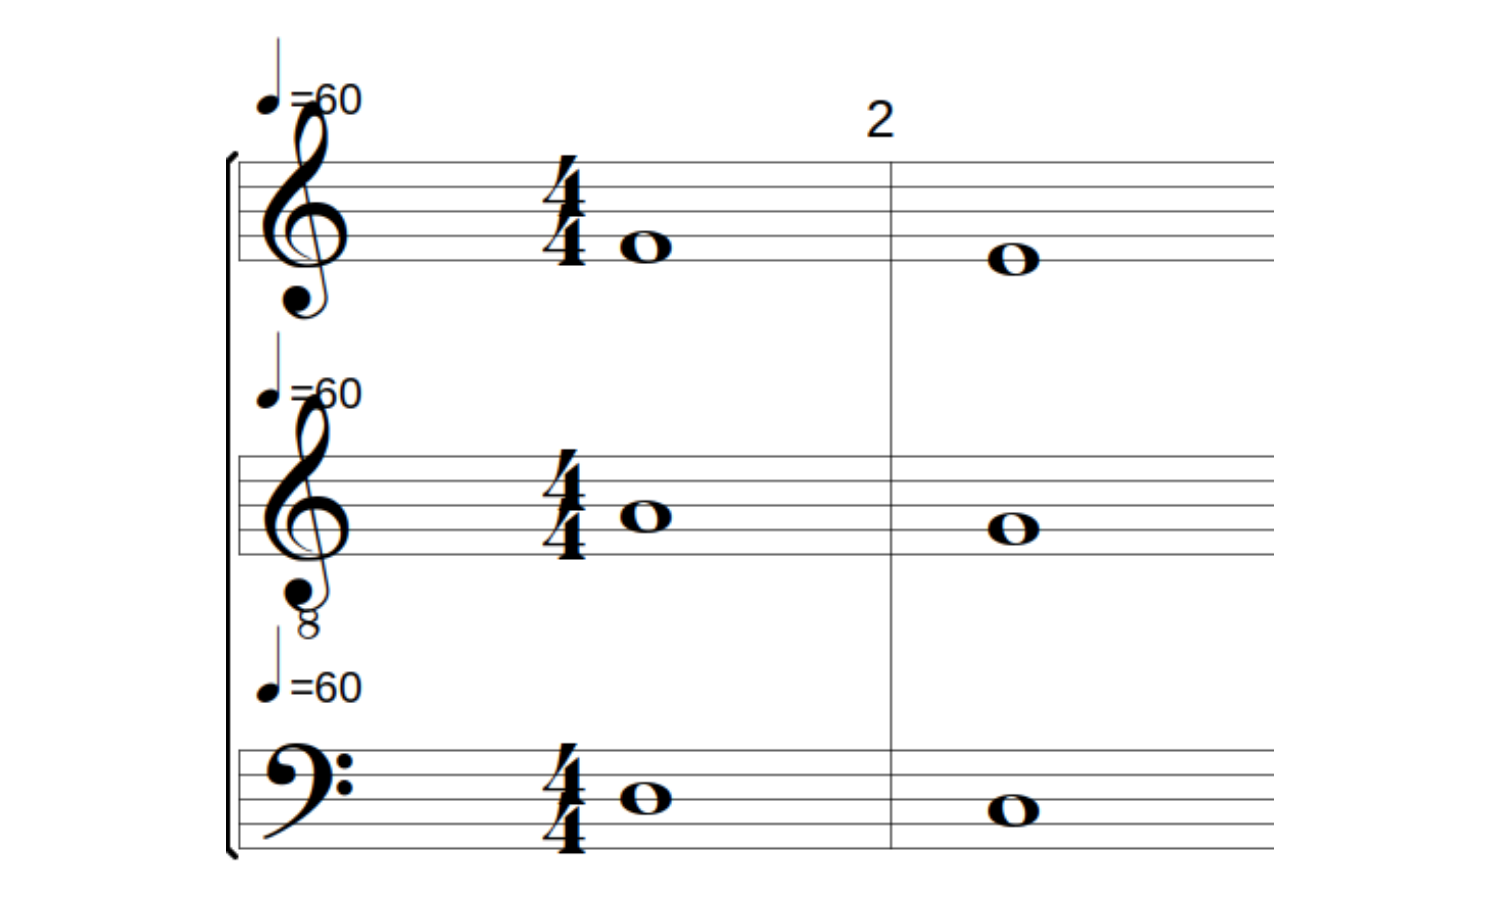
\includegraphics[width=\textwidth]{Images/successive-fifths.png}
    \captionof{figure}{Successive fifths - prohibited}
    \label{fig:successive-fifths-2}
    \end{minipage}
    \hfill
    \begin{minipage}{0.46\textwidth}
      \centering
      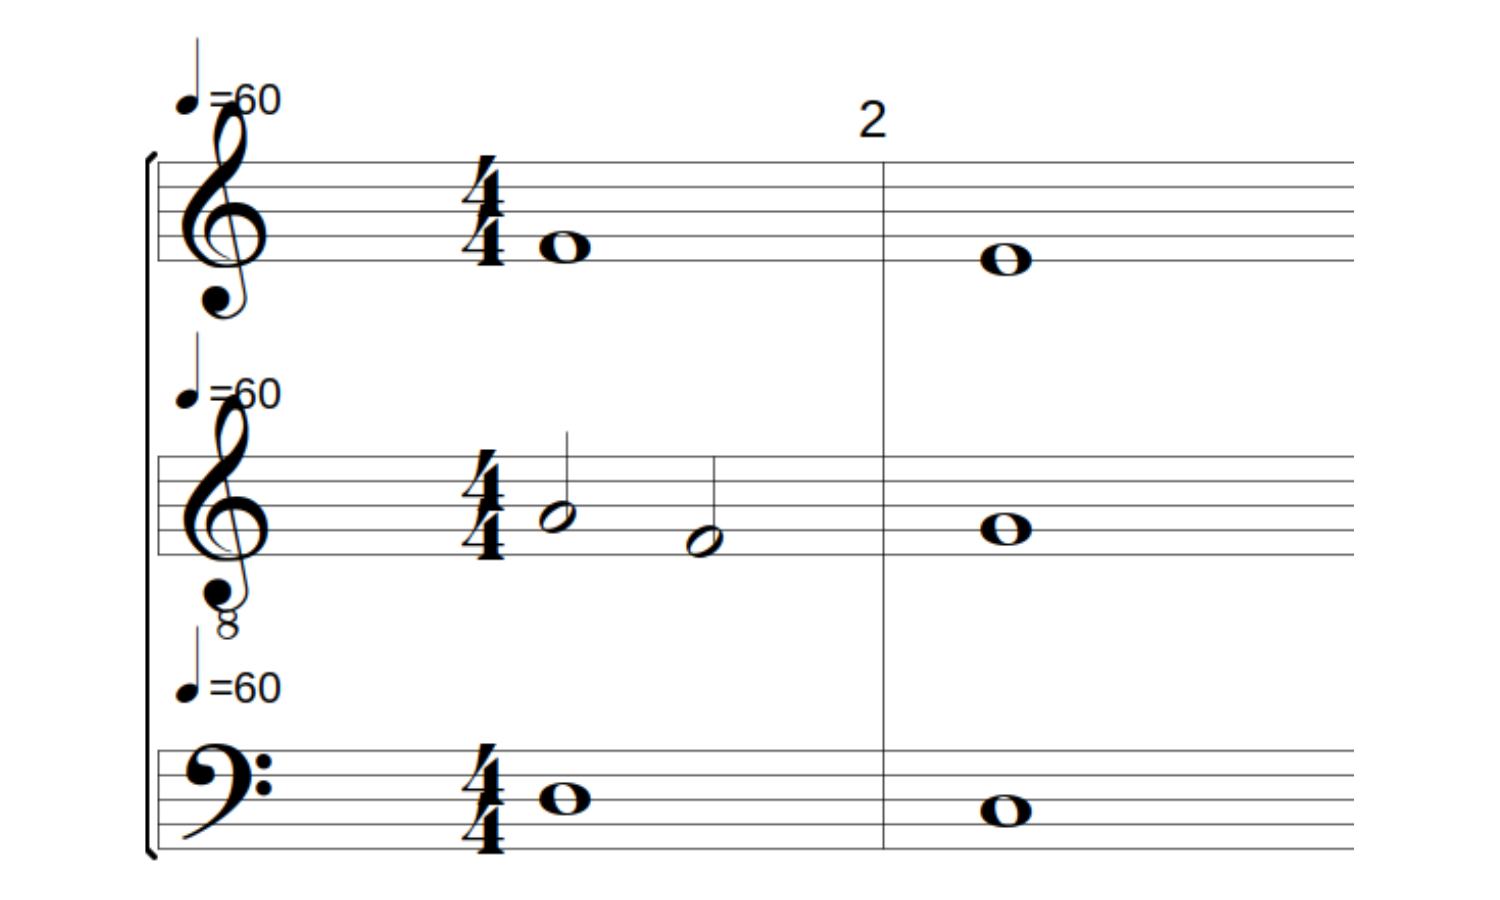
\includegraphics[width=\textwidth]{Images/successive-fifths-flanking-a-third.png}
      \captionof{figure}{Successive fifths separated by a third - valid}
      \label{fig:successive-fifths-2}
\end{minipage}
\end{enumerate}

\subsection{Formalisation into constraints}
\subsubsection{Harmonic constraints}
As discussed in \ref{formalisation-en-2nd}, no new harmonic rules were defined by Fux for the second species.

\subsubsection{Melodic constraints}
\begin{enumerate}[wide, label=\bfseries 2.M\arabic*]
\setcounter{enumi}{1} % Start from 2
    \item \textit{You might have a ligature from the third-to-last to the second-to-last measure or within the second-to-last measure.} \label{constraint:2nd-species-ligatures}    
    This is a relaxation of the two-voice rule \textbf{2.M2} "two consecutive notes cannot be the same". N[2, m-3] and N[0, m-2] are not covered anymore by the scope of this rule. The reason why this has been implemented a constraint relaxation instead than as a cost is because Fux seems not to say that there is any counterpart at ligaturing the fourth-to-last and the third-to-last notes: he doesn't say it is bad, he just says it is a new option.

    \begin{equation}
        \begin{aligned}
            &\forall j \in [1, m-1), \quad j \neq m-2:\\
            &(N[2, j-1] \neq N[0, j]) \land (N[0, j] \neq \land N[2, j])\\
            &\neg (N[2, m-3] = N[0, m-2]) \lor \neg(N[0, m-2] = N[2, m-2])
        \end{aligned}
    \end{equation}
\end{enumerate}

\subsubsection{Motion constraints}
\begin{enumerate}[wide, label=\bfseries 2.P\arabic*]
\setcounter{enumi}{1} % Start from 2
    \item \textit{Successive fifths on the downbeat are only allowed when they are separated by a third on the upbeat.} \label{constraint:succ-fifths-flanking-third}    
    \begin{equation} \begin{aligned}
    &\forall p_1, p_2 \in \{cf, cp_1, cp_2\}, \quad p_1 \neq p_2 \quad \forall j \in [0, m-2): species(p_1)=2 \implies \\
    &(H(p_1,p_2)[0, j] = 7) \land (H(p_1,p_2)[0, j+1] = 7) \\
    &\iff (H(p_1,p_2)[2, j] = 3) \lor (H(p_1,p_2)[2, j] = 4)
    \end{aligned} \end{equation}
\end{enumerate}

\section{Third species}
\subsection{Formalisation in English}\label{formalisation-en-3rd}
\subsubsection{Harmonic constraints}
\begin{enumerate}[wide, label=\bfseries 3.H\arabic*]
\setcounter{enumi}{4}
    \item \textit{The quarter notes must be coherent with respect to the whole notes.} \label{rule:concur-3rd}    
    \begin{quotation}
        "The quarters have to concur with the whole notes of the other voices."
        \textcite[p.91]{GaPEng}
    \end{quotation}
    When using the word "concur", Fux more than probably means "are put in relation", and not "are consonant". As for rule \ref{rule:concur-2nd} in the second species, where the half notes had to be \textit{concordant} with the \textit{cantus firmus}. It is not a rule by itself, Fux is only annunciating that some rules should be followed (i.e. the other constraints).

    \item \textit{In case the harmonic triad could not be used in the downbeat, it should be used in the second or third beat.} \label{rule:coherent}    
    \begin{quotation}
        "Take care whenever you cannot use the harmonic triad on the first quarter occurring on the upbeat, to use it on the second or third quarters."
        \textcite[p.91]{GaPEng}
    \end{quotation}

    This rule is quite clear and speaks for itself.
\end{enumerate}

\subsubsection{Melodic constraints}
Fux introduces no new melodic constraints for the third species.
\subsubsection{Motion constraints}
Fux introduces no new motion constraints for the third species.

\subsection{Formalisation into constraints}
\subsubsection{Harmonic constraints}
\begin{enumerate}[wide, label=\bfseries 3.H\arabic*]
\setcounter{enumi}{5}
    \item \textit{In case the harmonic triad could not be used in the downbeat, it should be used in the second or third beat.} \label{constraint:coherent}    

    This rule is quite clear and speaks for itself. Since this is not a strict rule but an advice, it was treated as a cost.

    \begin{equation} \begin{aligned}
            &\forall j \in [0, m-1) \colon \\
            &(H[1, j] \notin Cons_{h\_triad}) \land  (H[2, j] \notin Cons_{h\_triad})\\
            &\iff cost_{harmonic-triad-3rd-species}[j] = 1       
    \end{aligned} \end{equation}
\end{enumerate}




\section{Fourth species}
\subsection{Formalisation in English}\label{formalisation-en-4th}
\subsubsection{Structural constraints}
\begin{enumerate}[wide, label=\bfseries 4.S\arabic*]
\setcounter{enumi}{0}
    \item \textit{The fourth species is staggered by two beats.} \label{rule:delaying}    
    \begin{quotation}
        "The ligature is nothing but a delaying of the note following."
        \textcite[p.95]{GaPEng}
    \end{quotation}
    Fux here insists on the fact we have already discussed in \ref{nota-bene-4th-species}. The fourth species behaves as if its upbeat were the downbeat and its downbeat were the upbeat of the previous measure.

    \item \textit{All parts can become the lowest stratum somewhere in the composition.} \label{rule:tenor-might-take-place-of-bass}    
    \begin{quotation}
        "The tenor takes the place of the bass in the first measure - a thing that not only the tenor may do, but also the alto and even the soprano."
        \textcite[p.100]{GaPEng}
    \end{quotation}
    Fux speaks here about our concept of strata. The tenor can become the lowest stratum, just like the alto and the soprano may do. This is a fundamental concept of the generalization of Fux counterpoint to three voices, and has already been extensively discussed before (see section \ref{section:parts-and-strata}).
\end{enumerate}

\subsubsection{Harmonic constraints}
\begin{enumerate}[wide, label=\bfseries 4.H\arabic*]
    \setcounter{enumi}{4}
    \item \textit{Imperfect consonances are preferred over fifth intervals, which in turn are preferred over octaves.} \label{rule:prefer-fifths-over-octaves}    
    \begin{quotation}
        "The fifth is a perfect consonance, the octave a more perfect one, and the unison the most perfect of all; and the more perfect a consonance, the less harmony it has."
        \textcite[p.97]{GaPEng}
    \end{quotation}
    This rule is as clear as it gets.
\end{enumerate}

\subsubsection{Melodic constraints}
Fux introduces no new melodic constraints for the third species.

\subsubsection{Motion constraints}
\begin{enumerate}[wide, label=\bfseries 4.P\arabic*]
\setcounter{enumi}{2}
    \item \textit{Successive fifths are allowed when using ligatures.} \label{rule:successive-fifths-in-4th-species}    
    \begin{quotation}
        "[It would be impossible to remove] the ligatures because of another consideration, the immediate succession of several fifths."
        \textcite[p.95]{GaPEng}
    \end{quotation}
    By saying that it exists a rule that prohibits the succession of fifths (which is actually just a particular case of rule \ref{rule:succ-p-cons}, stating that you cannot have two successive perfect consonances) when there is no ligature, Fux is telling us in an indirect way that this rule is not applicable when there are ligatures. He further complements by saying "there is great power in ligatures - the ability to avoid or improve incorrect passages". 

    \item \textit{Resolving to a fifth is preferred over resolving to an octave.} \label{rule:resolving-to-fifths-rather-than-octaves}    
    \begin{quotation}
        "A dissonance that resolves to a fifth is more acceptable than a dissonance that resolves to an octave."
        \textcite[p.98]{GaPEng}
    \end{quotation}
    This rule could not be clearer.
    
    \item \textit{Stationary movement in the bass implies dissonance in the fourth species part.} \label{rule:dissonance-in-4th-species}
    \begin{quotation}
        "If I said that the first note of the ligature must always be consonant, that applies only to the instances in which the lower voice moves from bar to bar, but not the instances in which the bass remains on a pedal point, that is, in the same position. In such a case a ligature involving only dissonances is not only correct but even very beautiful."
        \textcite[p.98]{GaPEng}
    \end{quotation}
    The rule evoked here cancels the previous rule \textbf{4.H1W} that stated that all notes should be consonant. From now on, if the lowest stratum has a stationary movement, the corresponding delayed note in the fourth species must be a dissonance, instead of a consonance.    


    \item \textit{A note provoking a hidden fifth gets replaced by a rest.} \label{rule:hidden-fifths}
    \begin{quotation}
        "Here a hidden succession of two fifths occurs, which is easily perceptible to the ear and should be avoided in three part composition. This may be managed by using a rest in the alto."
        \textcite[p.98]{GaPEng}
    \end{quotation}
    Fux's uses the term 'hidden fifth' without any prior definition. It is therefore difficult to be sure of what he meant, since the traditional terms for such progressions are as vague and variable as the traditional rules that govern them. Nevertheless, most people seem to agree on the following definition of a 'hidden interval': a hidden fifth or hidden octave is when you approach a perfect fifth or perfect octave by direct motion. \cite[p.31]{piston1987harmony}. Looking closely at figures 137, 151 and 152 of the English version of \gap, this definition is consistent with Fux's interpretation.

    The point of the rule then is: if a solution leads to a hidden fifth, then the note that provokes the fifth is replaced by a rest. This rule is an \textit{a posteriori} rule: it applies after the solution has been found.
    The current rule thus complements the rule \ref{rule:successive-fifths-in-4th-species} (about successive fifths in fourth species) and the rule \ref{rule:direct-to-p-cons} (about direct moves to perfect consonances) without changing them.
    
    See figures \ref{fig:hidden-fifths-1} and \ref{fig:hidden-fifths-2}:

    \vspace{.5cm}
    \begin{minipage}{0.46\textwidth}
    \centering
    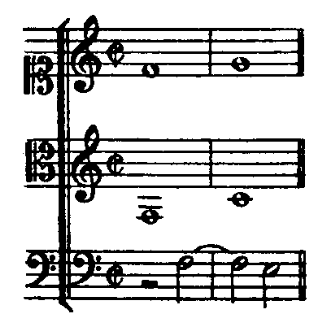
\includegraphics[width=\textwidth]{Images/hidden-fifths-1.png}
    \captionof{figure}{Invalid solution featuring hidden fifths}
    \label{fig:hidden-fifths-1}
    \end{minipage}
    \hfill
    \begin{minipage}{0.46\textwidth}
      \centering
      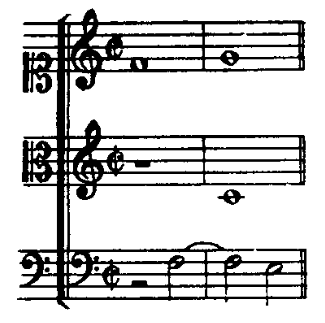
\includegraphics[width=\textwidth]{Images/hidden-fifths-2.png}
      \captionof{figure}{Valid solution replacing the hidden fifth by a rest.}
      \label{fig:hidden-fifths-2}
    \end{minipage}

\end{enumerate}

\subsection{Formalisation into constraints}\label{formalisation-c-4th}
\subsubsection{Harmonic constraints}
\begin{enumerate}[wide, label=\bfseries 4.H\arabic*]
    \setcounter{enumi}{4}
    \item \textit{Imperfect consonances are preferred over fifth intervals, which in turn are preferred over octaves.} \label{constraint:prefer-fifths-over-octaves}   
    \item  
    This rule is almost covered by the existing costs, as a perfect consonance has a cost of 1, where an imperfect consonance has a cost of 0. But Fux says not only that imperfect consonance should be preferred over perfect ones, he says that fifths should be preferred over octaves. This precision in the rule (fifth is better than octave) could be solved by either putting a cost of 2 to octaves and a cost of 1 to fifths, or to put the cost for fifth before the cost for octaves in the lexicographical array of costs, but this is discussed in the parts about costs (see \ref{costs}).

\end{enumerate}

\subsubsection{Motion constraints}
\begin{enumerate}[wide, label=\bfseries 4.P\arabic*]
\setcounter{enumi}{2}
    \item \textit{Successive fifths are allowed when using ligatures.} \label{rule:successive-fifths-in-4th-species}    

    The point of this rule is that Fux introduces an exception to \ref{rule:succ-p-cons}: successive fifths are allowed in the fourth species, thanks to the delaying it induces.

    We shall then amend rule \ref{rule:succ-p-cons} to only prohibit successive octaves, and rewrite it as:
    \begin{equation} \begin{aligned}
        &\forall p_1, p_2 \in \{cf, cp_1, cp_2\}, \quad p_1 \neq p_2 \quad \forall n \in \{0, 1\} \\
        &i_n := \,  
        \begin{cases}
            0 & \text{if } species(p_n) \neq 4\\
            2 & \text{if } species(p_n) = 4\\
        \end{cases}\\
        &\forall j \in [0, m-2) \colon H(p_1,p_2)[i_n, j] \neq 0 \iff H(p_1,p_2)[i_n, j+1] \neq 0
    \end{aligned} \end{equation}

    \item \textit{Resolving to a fifth is preferred over resolving to an octave.} \label{constraint:resolving-to-fifths-rather-than-octaves}    
    This is already treated by the rule \ref{rule:prefer-fifths-over-octaves}, as rule \ref{rule:prefer-fifths-over-octaves} implies the current rule (\ref{rule:resolving-to-fifths-rather-than-octaves}), as the fifth is preferred to the octave in any case.

    \item \textit{Stationary movement in the bass implies dissonance in the fourth species part.} \label{constraint:dissonance-in-4th-species}

    \begin{equation}
        \begin{aligned}
        &\forall j \in [0, m-1):\\
        &M(a) \neq 0 \iff H[2, j] \in Cons\\
        &M(a) = 0 \iff H[2, j] \in Dis
        \end{aligned}
        \label{eq:arsiscons} 
    \end{equation}        


    \item \textit{A note provoking a hidden fifth gets replaced by a rest.} \label{constraint:hidden-fifths}
    \begin{equation}
        \begin{aligned}
            &\forall j \in [1, m-1):\\
            &H[0, j] = 7 \land P[0,j] = 2 \iff N(0, j-1) = \emptyset  
        \end{aligned}
    \end{equation}


\end{enumerate}

\section{Fifth species}
No supplementary rules have been observed by Fux for the fifth species.

However, in order to have variety when composing with two fifth species counterpoints, it was decided to impose a rule that Fux never mentioned: knowing that the fifth species is just all other combined, not more than 50\% of the composition of the parts can be made using the same species for the same measure. This translates as:
\begin{equation}
\begin{aligned}
species(cp_1) = 5 = species(cp_2)  \iff \sum_{i=0}^{3} \sum_{j=0}^{m-1} (S(cp_1)[i,j] = S(cp_2)[i,j]) < \frac{s_m}{2}
\end{aligned}
\end{equation}
